\documentclass[12pt,a4paper]{article}
% Options possibles : 10pt, 11pt, 12pt (taille de la fonte) % oneside, twoside (recto simple, recto-verso) % draft, final (stade de d̩veloppement)
%\usepackage[utf8]{inputenc} % LaTeX, comprends les accents ! 
%\usepackage[T1]{fontenc} % Police contenant les caract̬res fran̤ais \usepackage[francais,english]{babel} % Placez ici une liste de langues, la 
%\usepackage{gensymb} % derni̬re ̩tant la langue principale 
\usepackage{braket} 
\usepackage[a4paper]{geometry}% R̩duire les marges % 
\pagestyle{headings} % Pour mettre des ent̻tes avec les titres
 \usepackage[all]{xy} 
 \usepackage{graphicx} 
\usepackage{tabularx}
\usepackage[utf8]{inputenc}
\usepackage[demo]{graphicx} 
\usepackage{siunitx}
\usepackage[nottoc]{tocbibind}
%\usepackage{cite}
%\usepackage[backend=biber,hyperref=true,backref=false,sorting=none,style=nature,citestyle=numeric,maxcitenames=100,maxbibnames=1000]{biblatex}
\usepackage[hidelinks]{hyperref}
\usepackage[backend=bibtex, sorting=none,hyperref=true,style=nature,maxcitenames=99,maxbibnames=999]{biblatex}
%\bibliographystyle{abbrv}
\bibliography{biblio}

\usepackage{tikz}
\usetikzlibrary{shapes,arrows}

\tikzstyle{block} = [rectangle, draw, fill=blue!60, 
    text width=25em, text centered, rounded corners, minimum height=1em]
\tikzstyle{line} = [draw, -latex']
%\bibliography{biblio.bib}       
\phantomsection
\usepackage{amsmath}
\usepackage{comment} 
\usepackage{xcolor}
\usepackage{float} % des sections en haut de page 
\usepackage[left=3cm,right=2cm,top=3cm,bottom=2cm]{geometry}
\usepackage{fancyhdr} 
\usepackage[utf8]{inputenc} % LaTeX, comprends les accents ! 
\fancyhf{}
\cfoot{\thepage}
\pagestyle{fancy} 
\begin{titlepage}
\title{Assessment of COF stacking} % Les param̬tres du titre� : titre, auteur, date 
\author{LMSO \\ 
\\ Prof. Berend Smit \\ 
\\ Andres Ortega Guerrero\\ 
\\ Viterbo Victor
\\
\\} % La date n'est pas requise (la date du % jour de compilation est utilis̩e en son % absence)
%\date{August, 31 2018}
\sloppy % Ne pas faire d̩border les lignes dans la marges

\cfoot{\thepage}
\begin{document} 
\maketitle 
\begin{figure}[H] 
\includegraphics[width=100mm]{EPFL_Logo.pdf}
\centering 
\end{figure}
\clearpage 
\end{titlepage}
\tableofcontents
\clearpage

\section{Introduction}

Covalent Organic Frameworks are a novel class of materials made from self assembled small organic molecules, imagined and first synthesised by C\^{o}t\'e et al. in 2005\cite{cote_porous_2005}. First COFs were two-dimensional polymers formed by a dehydration condensation reaction of boronic acid ($RB(OH)_2$) into boroxin rings ($R_3(BO)_3$). Latter, more diverse ligands and structures were elaborated, by adding vertical linkers to yield three- dimensional polymers or the use of triazine or imine condensation instead of boronic ones.

These materials drew an increasing interest because of their lightness, porosity and optical properties all the while being easy to functionalise, and are therefor excellent candidates for gas separation and storage, electrochemistry, heterogeneous catalysis, and light harvesting; but this very high tunability of the material also makes the number of ligand combination extremely large. 

Since experimental chemistry would be unable to assess such amounts of structures, in part due to technical limitations like the high sensitivity to defects of x-ray diffraction, and the low crystallinity of theses materials. In some cases High Resolution Transmission Electron Microscopy was able to give some property like the single layer vector but is unable to asses its stacking. Hence, the advantage of using computational chemistry becomes obvious : it makes it possible to test for a property in a systematic fashion among a very large number of materials without the need for synthesis. 

Since COFs' properties are strongly dependant on their stacking structure, wether it be geometric ones for gas adsorption and separation or electronic ones for optoelectronic processes, the first step of the calculation is to compute it as accurately as possible to then converge to an exact structure and obtain more complex properties of the material. The problem is now that accurate calculations are very expensive machine-time-wise and a fine x,y,z offset grid is necessary to achieve reasonable accuracy, especially when this number of grid-points are put together with the number of materials to test. To alleviate this cost, the solution chosen here is to make a first estimation of the structure using a method as cheap as possible that still gives a useful starting point for more in-depth optimisation. In this setting, the work detailed below aims at finding the best compromise between calculations that are too expensive to be interesting as a pre-screener and the ones that are not accurate enough to give a useful initial guess for the rest of the treatment. With this idea in mind, different computational technics were tested on a diverse set of COFs in order to evaluate the complexity of calculations needed to achieve reasonable precision. These technics, from simplest to most elaborate are : the Lennard-Jones potential, Lennard-Jones and Coulombic interactions, DFTB+ \cite{aradi_dftb+_2007} and GFN2-xTB \cite{grimme_robust_2017}\cite{bannwarth_gfn2-xtb_2019}.

Furthermore, by scanning all possible x,y,z offsets from one layer to the next it is possible to asses the crystallinity of the material : a steep, smooth potential would yield high crystallinity while irregularities and flatness in the Potential Energy Surface would yield lower crystallinity. This can be of the utmost importance when aiming at applications like light harvesting where irregularity in the crystalline structure can strongly impair the material's efficiency.




\section{Methodology}

%\subsection {Workflow Overview}

\subsection{General Considerations}

To avoid artefacts, each COF was studied using a naive structure (theoretical bond-angles and bond-lengths) and using this same structure relaxed using CP2K's geometry and cell optimisation.


\begin{figure}\centering
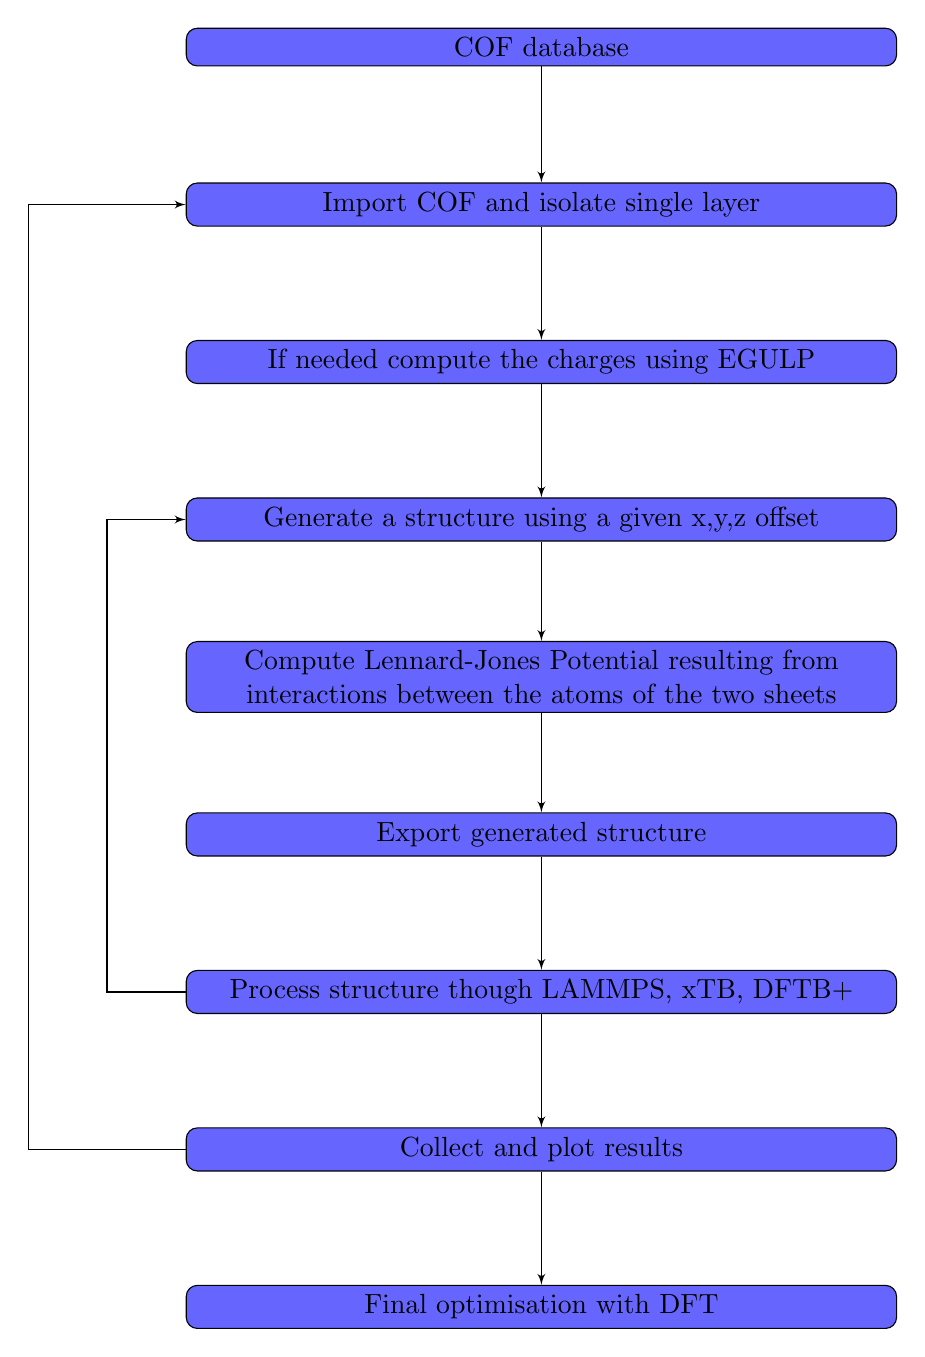
\begin{tikzpicture}[node distance = 2cm, auto]\centering
    % Place nodes
    \node [block] (db) {COF database};
    \node [block,below of=db] (import) {Import COF and isolate single layer};
    \node [block, below of=import] (charges) {If needed compute the charges using EGULP} ;
    \node [block, below of=charges] (struct_gen) {Generate a structure using a given x,y,z offset};
    \node [block, below of=struct_gen] (LJ) {Compute Lennard-Jones Potential resulting from interactions between the atoms of the two sheets};
    \node [block, below of=LJ] (export) {Export generated structure};
    \node [block,below of=export] (funcall) {Process structure though LAMMPS, xTB, DFTB+};
    \node [block, below of=funcall] (collect) {Collect and plot results};
    \node [block, below of=collect] (DFT) {Final optimisation with DFT};
    
  \path [line] (db) -- (import);
  \path [line] (import) -- (charges) ;
  \path [line] (charges) -- (struct_gen);
  \path [line] (struct_gen) -- (LJ);
  \path [line] (LJ) -- (export);
  \path [line] (export) -- (funcall);
  \path [line] (funcall) -- (collect);
  \path [line] (collect) -- (DFT);
  \path [line] (funcall.west) -- ++(-1,0) -- ++ (0,6) -- ++(1,0)  ;
  \path [line] (collect.west) -- ++(-2,0) -- ++ (0,12) -- ++(2,0)  ;
\end{tikzpicture}
\caption{\textit{Overview of the workflow in the setting of this project}}
\end{figure}


\subsection{Lennard-Jones}
%The Lennard-Jones potential is a classical approximation of non-binding interactions where interaction potential between two elements i and j is given by :
%$$E_{LJ}=4\epsilon_{ij}\left[\left(\frac{\sigma_{ij}}{r_{ij}}\right)^{12}-\left(\frac{\sigma_{ij}}{r_{ij}}\right)^{6}\right]$$
%where and $\epsilon_{ij}$ and $\sigma_{ij}$ are pair-specific parameters. 
%The positive part sands for the repulsion that results from the Pauli exclusion principle and the negative one for the coulombic attraction. The exponents were chosen for computational simplicity.
To asses the complexity of phenomenon involved in the stacking process of COFs, we used the Lennard-Jones potential, which is among the simplest classical approximations for computational chemistry to simulate the Van der Waals interactions. It relies on only two parameters :  the depth and the distance to the nucleus of the well. The parameters used were the Universal Force Field parameters from Rapp\'e et al. \cite{rappe_uff_1992}. Since these parameters are element-specific, mixing rule is needed to combine the parameters. In our case, the Lorentz-Berthelot \cite{lorentz_ueber_1881} mixing rules  were used, as it is the simplest and most widely used one, although it have been reported to fail in some very specific cases. It reads as follow :
$$ \sigma_{ij}=\sqrt{\sigma_i\sigma_j}   $$ and $$ \epsilon_{ij}=\frac{\epsilon_i + \epsilon_j}{2}$$
where indices i denote an element-specific parameter for element i, and incices $ij$ a pair-specific parameter. $\sigma_i$ and $\epsilon_i$ are the distance to $E_{LJ}=0$ from the nucleus and the depth of the well respectively.
%The parameter used are the Universal Force Field  ones
The tail correction used here was the truncated-shifted potential where the potential at cutoff is added to ensure a smooth potential at cutoff.
To lower the computational cost, only interactions between atoms of different sheets were computed.

\subsection{Charge Calculations}

For the experimental structures, no charges where given and where hence computed for a single sheet using the charge equilibration Qeq from EGULP subroutine \cite{kadantsev_fast_2013}. This method is also based on the Universal Force Field's parameters. The core principle behind this method is to use a second-order Taylor expansion, truncated to the second order, of the charge dependant energy ($E(Q)$)\cite{rappe_charge_1991} :
$$E_A(Q)=E_{A0}+Q_A\left(\frac{\partial E}{\partial Q}\right)_{A0}+\frac{1}{2}Q_{A0}^2\left(\frac{\partial^2 E}{\partial Q^2}\right)_{A0}$$
This parametrisation makes this problem computationally cheap by avoiding to go through a long and tedious quantum processing of the system and hence fast charge calculations.

Unfortunately, this method was not robust enough and showed some unphysical behaviours, among other yielding strongly asymmetric charge distribution in a symmetric system, or yielding positively charged Fluorine in a fluorinated benzene on a single sheet (to exclude interactions between layers).

This indicates that the systems under study here needs a more complete treatments in order to obtain the equilibrated charges. An in-depth analysis of the charges as computed by DFTB+ was also performed to asses the strength of the interactions between layers in the repartition of charges within a layer. This may enable one to estimate the necessity to recompute the charges for every stacking configurations or not. 

\subsection{Coulombic Potential and Ewald Summation}

The Coulombic potential is given by :
$$E_c=k_e\frac{q_iq_j}{r_{ij}}$$
where $k_e$ is the Coulomb's constant, $q_i$ and $q_j$ the charge of the atoms i and j respectively, and $r_{ij}$ the distance between the two atoms. 
Since this potential converges slowly in periodic systems, it is important to take into account the long range interactions. A natural way to do so would be a very high cutoff but it would strongly increase the computational cost drastically. To tackle this problem, one can take advantage of the periodicity of the system and compute separately the short range interactions by summing them in real space and sum the long range interactions in reciprocal space : this is known as the Ewald summation \cite{lee_ewald_nodate}, which is a special case of the Poisson summation. The charge density is split as follow :
$$\rho_i(r) = \rho_i^S(r)+\rho_i^L(r)$$
where $\rho_i^S(r)$, the short range function is as follow
$$\rho_i^S(r) = q_i\delta(r-r_i)-q_iG_\sigma(r-r_i)$$
and $\rho_i^L(r)$, the long range function :
$$\rho_i^L(r)=q_iG_\sigma(r-r_i)$$
with 
$$G_\sigma=\frac{1}{(2\pi\sigma^2)^{3/2}}exp\left[-\frac{|r|^2}{2\sigma^2}\right]$$
The substitution above is equivalent to adding and subtracting a guassian function around each point charge, described by the dirac delta function. This will shield long range interactions in the short-range function and the long range 
We then integrate the short range function in real space and the long range in reciprocal space.
This technic allows for fast convergence of the Coulombic potential in periodic systems. 

For this project, LAMMPS (Large Scale Atomic/Molecular Massively Parallel Simulator)\cite{plimpton_fast_nodate} was used for its implementation of the Ewald Summation. 

%In order to be able to grasp the principle of the two following technics, it is important to first go through the principle that is the foundation of almost all newly developed technics : the Density Functional Theory. It mostly lies on the Hohnenberg-Kohn theorem that states that : 

%\textit{In a finite, interacting N-electron system with a given particle-particle interaction, there exists a one-to-one correspondence between the external potential v(r) and the ground state-density $n_0[v](r)$. In other words, the external potential is a unique functional of the ground-state density, $v[n_0](r)$, up to an arbitrary constant}\cite{ullrich_time-dependent_2011}. 

%With :
%$$n_0[v](r)=\sum_i|\Psi_i(r)|^2$$

%This equivalence simplify greatly the calculations and enabled computational chemistry to start tackling problems of a complexity that was before out of reach. The difficulty now resides in finding an efficient functional to compute the energy and other system properties.



% It lies on the equivalence between treating $N$ one-electron wavefunction $\Psi_i$ and one $N$ electron density function $n(r)$ with :
%where the summation is done over the $i$ electrons.
%It is based on the fact that a non-degenerate ground state of a $N$ electron system is fully determined for a given external potential, and hence :
%$$V_{ext} \leftrightarrow n(r)$$
%The first Hohnenberg-Kohn theorem goes further and state that a unique functional of the density function $n(r)$ exists and yield the energy of the system.
%The second Hohnenberg-Kohn theorem state that the true density function of the ground state is the one that minimise the energy.
%Together these theorems are the foundation of DFT calculations.


 
\subsection{Geometry, Frequency, Non-bonding - Tight Binding method (GFN2-xTB)}

GFN2-xTB is a method that approximates the Density Functional Theory that uses parameters that are atom-specific. It is mostly designed for vibrational analysis, geometry optimisation and non covalent interactions (the latest being the one we are interested in here).
The theory it relies on reads as follow, starting from the total energy :
$$E=E_{el} + E_{rep} + E_{disp} + E_{XB}$$
with $E_{rep} $ the repulsion energy, $E_{disp}$ the dispersion energy and $E_{XB}$ the halogen bonding and $E_{el}$ the electronic potential is the third-order-truncated Taylor expansion of the potential :
$$E_{el}=\sum_i^{occ}n_i\braket{\Psi_i|H_0|\Psi_i}+\frac{1}{2}\sum_{A,B}\sum_{l(A)}\sum_{l'(B)}
p_{l}^Ap_{l'}^B\gamma_{AB,ll'}+\frac{1}{3}\sum_A\Gamma_Aq_A^3-T_{el}S_{el}$$
The first order therm is simply the energy associated with each electron in its Molecular Orbital, the second order and third order term are the SCC contribution taking only in account diagonal terms and the additional term $T_{el}S_{el}$ is the electronic thermal-entropic terms.
 $\Psi_i$ is the valence Molecular Orbital with occupation $n_i$, $H_0$ the zero-order Hamiltonian, $q_A$ the Mulliken charges of atom $A$, $\Gamma_A$ the derivative of the Hubbard parameter $\eta_A$,$l$ and $l'$ are the electronic shells of atoms $A$ and $B$ respectively and $p_l^A$ the charge distribution on atom $A$'s shells with angular momentum $l$  and $\gamma_{AB,ll'}$ is a Coulombic space-dependant damping factor.
The xTB was run using the D3 dispersion correction and the SPME (Smooth Particle Mesh Ewald) summation, the Hessian matrix was estimated using the Broyden mixing scheme, for at least 8 steps before alternating with the Direct Inversion in the Iterative Subspace \cite{pulay_convergence_1980}\cite{pulay_improved_1982}\cite{shepard_comments_2007}.

\subsection{DFTB+}
The Density Functional-Based Tight Binding (DFTB) is a more heavily parametrised method. It relies on an expansion around the density functional energy using a non self-consistent Hamiltonian from interactions between Atomic Orbitals.
%It is based on the spin-polarized Hamiltonian below :
%$$\hat{H}_{\mu\nu}^\sigma = \braket{\phi_\mu|\hat{H_0}|\phi_\mu}+\frac{1}{2}S_{\mu\nu}\sum_C\sum_{l''\inC}(\gamma_{Al,Cl''}+\gamma_{Bl',Cl''})\Delta q_{C_{l''}}$$
%$$\pm \frac{1}{2}S_{\mu\nu}\left(\sum_{l''\in A}W_{All''}m_{Al''}+\sum_{l''\in B}W_{Bll''}m_{Bl''}\right)$$
%The first term being the non-SCC Hamiltonian, the second term is the SCC contribution,



\subsection{Density Functional Theory}

Density Functional theory is a technic that lies on the physical equivalence of a set of $N$ one-electron wavefunction $\Psi(r)$ and the sum of its position dependant module $n(r)$, the density function. A functional is then applied on the density function to extract observables as the energy. It was here used as the last stage of our process in oder to obtain the reference COF stacking starting from each technic's guess in order to asses its accuracy. 
The PBE (Perdew$-$Burke$-$Ernzerhof) functional, a nonempirical GGA (Generalized Gradient Approximation) functional. In addition, the DFT-D3 correction term for dispersion forces (London Forces) was used, and set to included the $9^{nth}$ order term, since theses play a key role in the non-bonding interactions that will determine the optimum stacking. For all elements, including Hydrogen, a Gaussian Double-Zeta function was used for the basis set \cite{vandevondele_gaussian_2007} to mimic accurately polarisation.





\begin{figure}[H]  \centering
\includegraphics[width=140mm,angle=0]{../2-atom-LJ/2-atom-with-analytical.pdf} 
\caption{\textit{Analytical, Python computed and LAMMPS computed LJ potential for two B atoms}}
\end{figure}









\begin{comment}
\begin{figure}[H]
\begin{tabularx}{\textwidth} { >{\centering \arraybackslash}X| >{\centering \arraybackslash}X| >{\centering \arraybackslash}X| >{\centering \arraybackslash}X| >{\centering \arraybackslash}X| >{\centering \arraybackslash}X| >{\centering \arraybackslash}X}
Scan Rate [mV/s] & \multicolumn{2}{c|}{$\frac{i^{Ox}}{i^{Red}} [-]$} & \multicolumn{2}{c|}{$\frac{i^{Ox}_{25}}{i^{Ox}} [-]$} & \multicolumn{2}{c|}{$\Delta E_p  [mV]$} \\
\hline
\hline
& Au & Ni & Au & Ni & Au & Ni \\
\hline
\hline
25 & 1.056 & 1.059 & 1 & 1 & 74 & 94\\
\hline
50 & 1.059 & 1.114 & 1.017 & 1.010 & 74 & 98\\
\hline
75 & 1.062 & 1.131 & 1.024 & 1.021 & 72 & 104\\
\hline
100 & 1.068 & 1.155 & 1.025 & 1.033 & 74 & 110\\
\hline
150 & 1.073 & 1.196 & 1.029 & 1.063 & 74 & 120\\
\hline
200 & 1.075 & 1.238 & 1.030 & 1.076 & 74 & 126\\
\hline
300 & 1.077 & 1.336 & 1.029 & 1.107 & 76 & 138\\
\end{tabularx}
\caption{\textit{From left to right: scan rate, ratio of the oxidative peak height over the reductive peak height, normalised oxidative peak height at a given scan rate over the normalised peak height at 25 mV/s, peak to peak separation.}}
\end{figure}
\end{comment}
%\bibliography{biblio}
\printbibliography
\end{document}
